% !TEX root = ../Masters.tex
\chapter{Plants Used in Survey}
\label{app:survey-plants}

\begin{figure}
    \centering
    \begin{subfigure}{0.48\textwidth}
        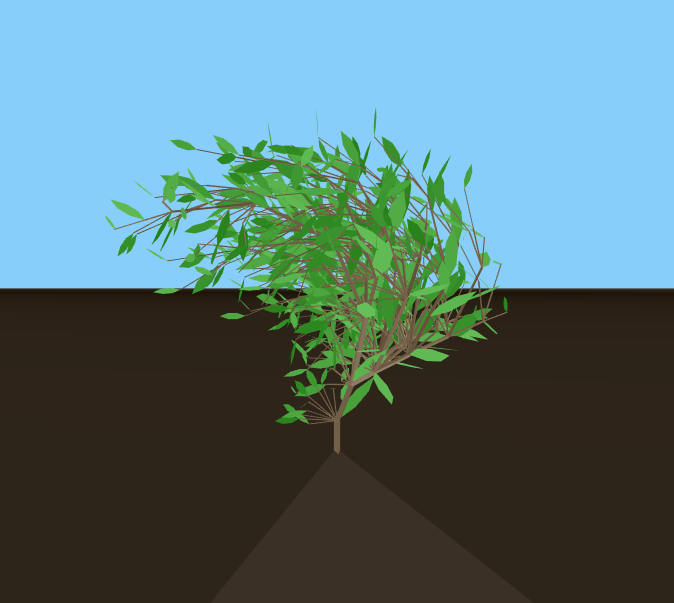
\includegraphics[width=\textwidth]{figures/plant-97}
        \caption{Survey plant 0.97}
    \end{subfigure}
    ~
    \begin{subfigure}{0.48\textwidth}
        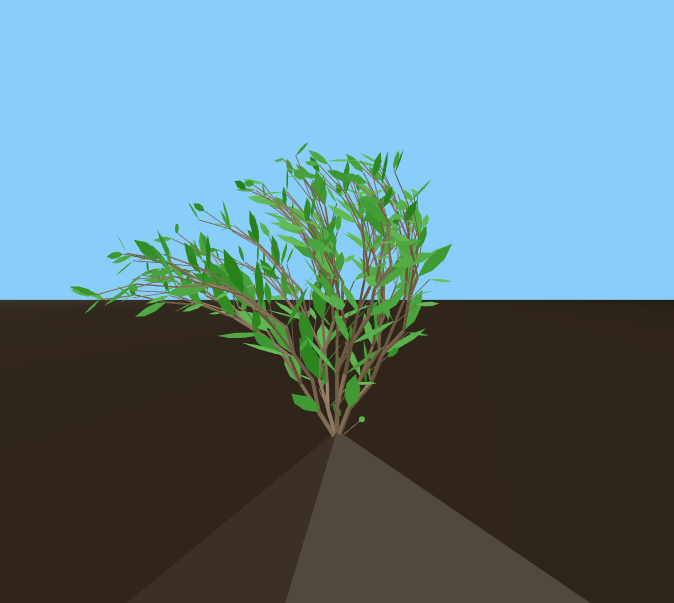
\includegraphics[width=\textwidth]{figures/plant-91}
        \caption{Survey plant 0.91}
    \end{subfigure}
    \\
    \begin{subfigure}{0.48\textwidth}
        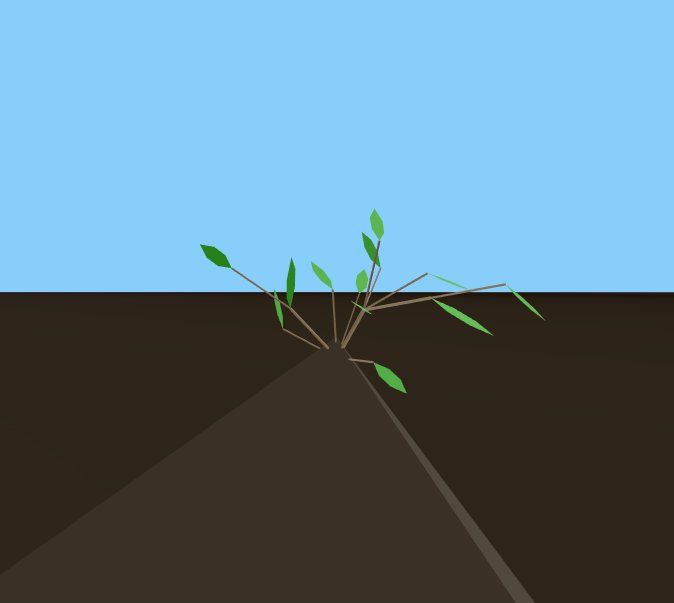
\includegraphics[width=\textwidth]{figures/plant-84}
        \caption{Survey plant 0.84}
    \end{subfigure}
    ~
    \begin{subfigure}{0.48\textwidth}
        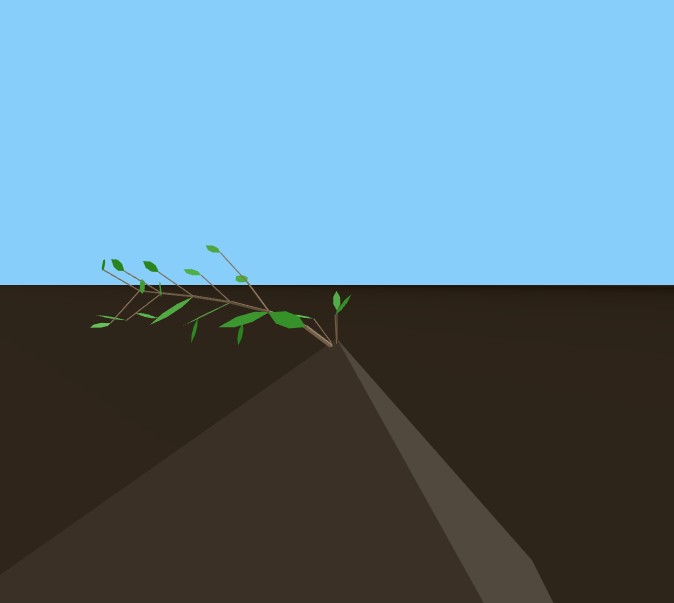
\includegraphics[width=\textwidth]{figures/plant-78}
        \caption{Survey plant 0.78}
    \end{subfigure}
    \\
    \begin{subfigure}{0.48\textwidth}
        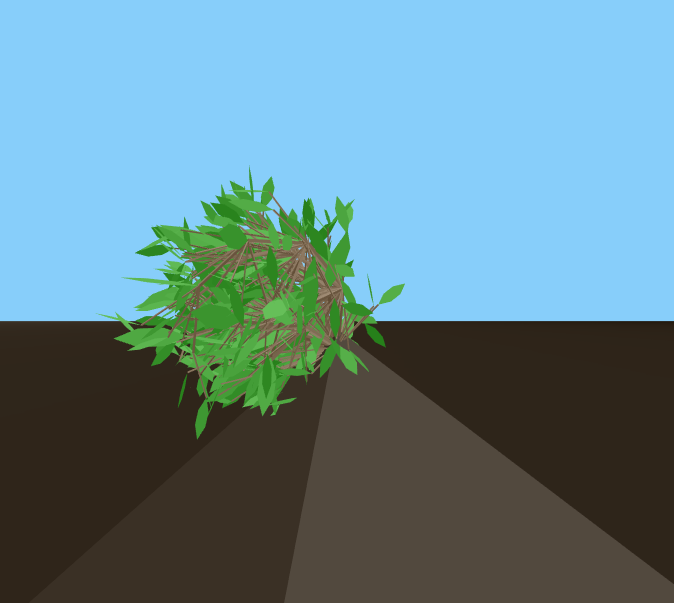
\includegraphics[width=\textwidth]{figures/plant-72}
        \caption{Survey plant 0.72}
    \end{subfigure}
    ~
    \begin{subfigure}{0.48\textwidth}
        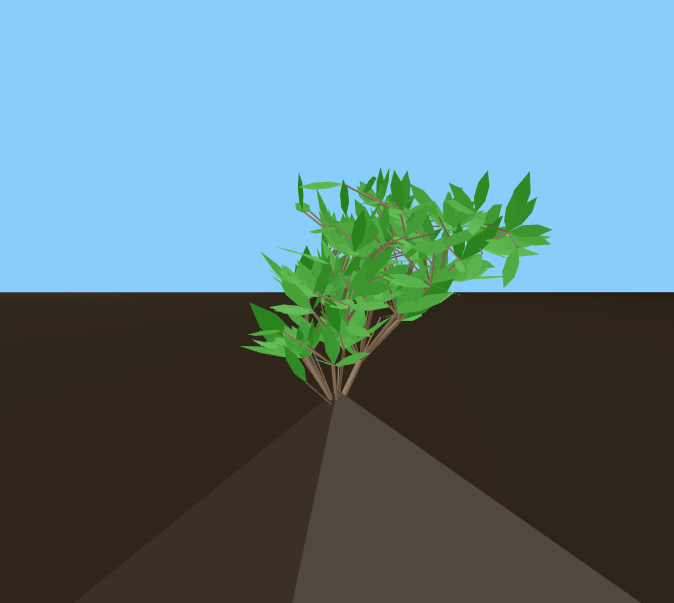
\includegraphics[width=\textwidth]{figures/plant-65}
        \caption{Survey plant 0.65}
    \end{subfigure}
\end{figure}
\begin{figure}
    \centering
    \begin{subfigure}{0.48\textwidth}
        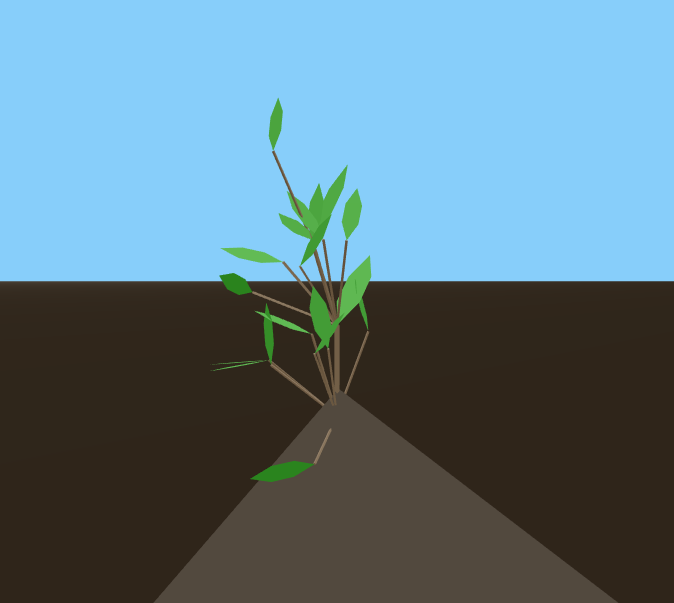
\includegraphics[width=\textwidth]{figures/plant-59}
        \caption{Survey plant 0.59}
    \end{subfigure}
    ~
    \begin{subfigure}{0.48\textwidth}
        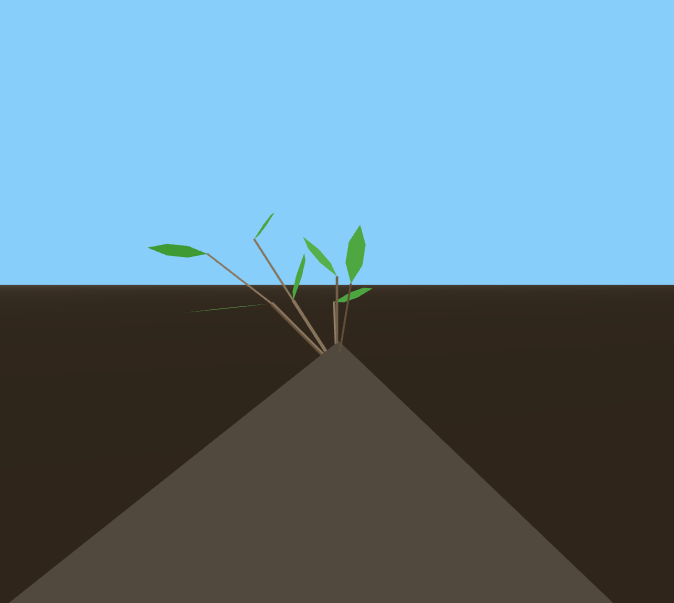
\includegraphics[width=\textwidth]{figures/plant-53}
        \caption{Survey plant 0.53}
    \end{subfigure}
    \\
    \begin{subfigure}{0.48\textwidth}
        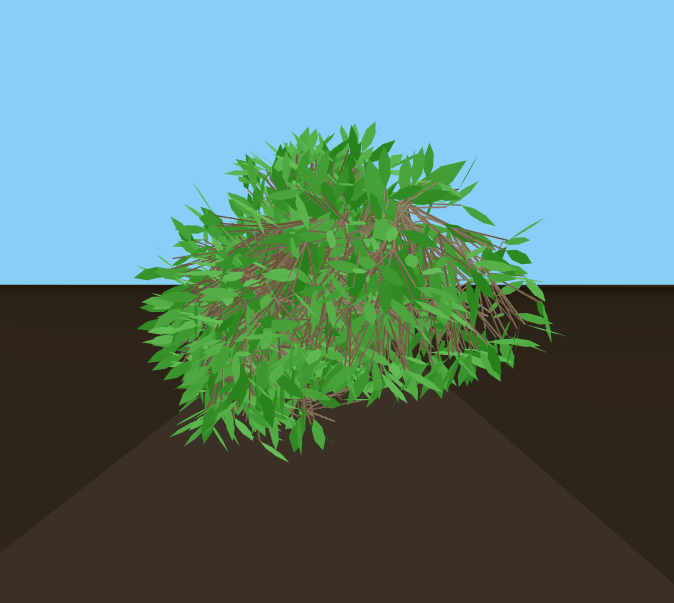
\includegraphics[width=\textwidth]{figures/plant-46}
        \caption{Survey plant 0.46}
    \end{subfigure}
    ~
    \begin{subfigure}{0.48\textwidth}
        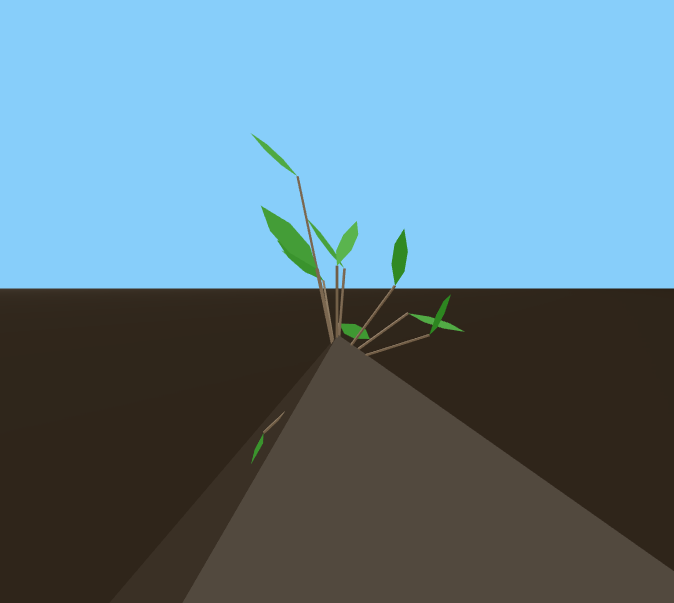
\includegraphics[width=\textwidth]{figures/plant-40}
        \caption{Survey plant 0.40}
    \end{subfigure}
    \\
    \begin{subfigure}{0.48\textwidth}
        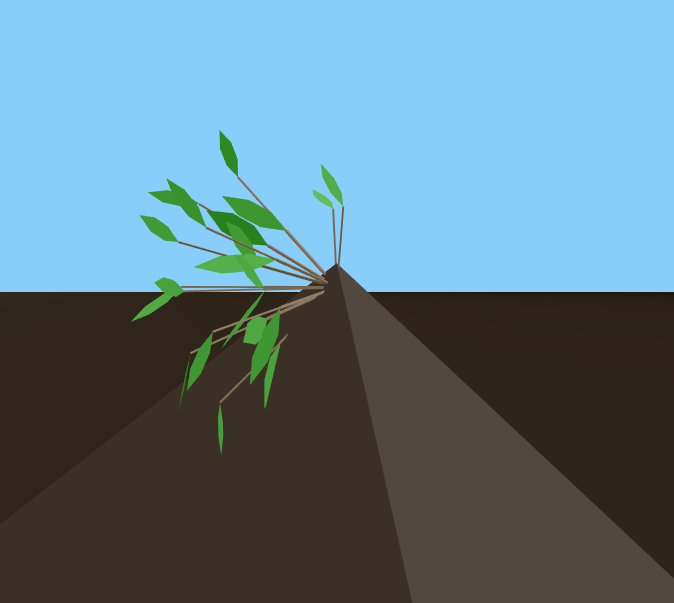
\includegraphics[width=\textwidth]{figures/plant-34}
        \caption{Survey plant 0.34}
    \end{subfigure}
    ~
    \begin{subfigure}{0.48\textwidth}
        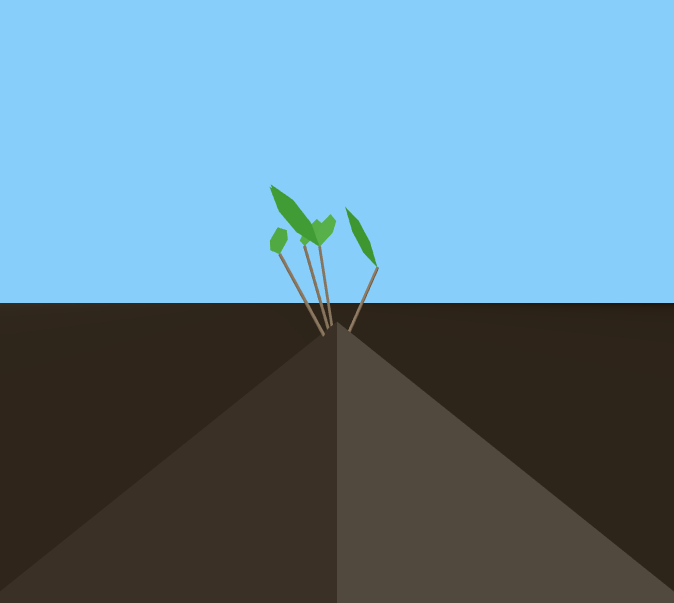
\includegraphics[width=\textwidth]{figures/plant-27}
        \caption{Survey plant 0.27}
    \end{subfigure}
    \ContinuedFloat
    \caption[All plants used in the survey]{All plants used in the survey, in descending rank order. Their name is equal to their fitness score.}
    \label{fig:survey-plants}
\end{figure}
